\documentclass[conference]{IEEEtran}
\IEEEoverridecommandlockouts

\usepackage{cite}
\usepackage{amsmath,amssymb}
\usepackage{graphicx}
\usepackage{booktabs}
\usepackage{algorithm}
\usepackage{algpseudocode}
\usepackage{url}
\usepackage[hidelinks]{hyperref}

\begin{document}

\title{When Not to Retrain: An Operation-Count Study of Cheap Repairs,
Spurious Alarms, and Delayed Action in Drift Adaptation}

\author{Author names --- United International University}

\maketitle

\begin{abstract}
Recent work reports energy savings from retraining only when drift is detected,
provided a reliable detector is in place. We examine that condition.
We measure what happens \emph{after} a detector fires, with
operation counts for training and for inference: a frozen
grid of 500 runs (5 streams, 4 model families, 5 policies, 5 seeds), a replicate
grid under a second detector, and an oracle executing every action at every alarm. A cost-ordered policy that tries the cheap repair
first does not win. It is less accurate than always rebuilding (median $-1.3$
points of mean prequential accuracy, balanced on multi-class), not reliably
cheaper than a fixed schedule, and half its rebuilds are forced by its own
minimum-window guard. On the two streams where we ran the oracle (Elec2,
Covertype; ADWIN), roughly 80\% of its advantage comes from skipping alarms. On
INSECTS-abrupt, the stream with published change points, only 27\% of ADWIN
alarms fall within 1{,}000 rows of one. XGBoost warm-start repairs permanently
raise per-prediction inference cost; the Random Forest repair does not. A
confirm-before-acting rule, judged against rules fixed in advance, improves
balanced accuracy but fails our cost and safety rules. We count operations, never joules.
\end{abstract}

\begin{IEEEkeywords}
concept drift, model retraining, drift detection, cost accounting, measurement study
\end{IEEEkeywords}

\section{Introduction}

A deployed model decays as the data shifts under it. The usual remedy is to watch
a drift detector and retrain whenever it fires, for as long as the model is in
service. That loop runs for the life of the system, so its cost keeps
accumulating while the initial training is paid once.

Poenaru-Olaru et al.~\cite{poenaruolaru2025} measure this and report that
retraining on recent data alone can use up to 25\% less energy, and that
drift-triggered retraining can save up to 40\% ``provided a reliable data change
detector is in place.'' We take that conditional clause as our subject. We do not
propose a better detector, and we do not propose a better repair. We ask what the
condition is worth on standard benchmarks: how much of the gain survives once the
alarms are examined, and where the operations actually go.

Our answer is that most of the available gain comes from \emph{not acting} on
alarms, and that a repair which looks cheap in training operations can raise the
cost of every prediction that follows it.

\textbf{Contributions.}
\begin{enumerate}
\item \textbf{A cost-accounted evaluation setup.} Hardware-independent operation
counts for training \emph{and} inference; a frozen 500-run grid (5 streams
$\times$ 4 families $\times$ 5 policies $\times$ 5 seeds) replicated under a
second detector; and a full-information oracle with a per-branch decomposition.
\item \textbf{A negative result for cost-ordered ``try cheap repair first''
adaptation.} The selector is not the best policy; cheap repairs fail in
family-specific ways, inert for Random Forest and Gaussian NB and overwriting for
SGD and XGBoost; and small post-alarm windows trigger guard-forced rebuilds.
\item \textbf{Alarm validity under cost.} Only 27\% of ADWIN alarms on
INSECTS-abrupt fall within 1{,}000 rows of a published change point; 40\% (ADWIN)
and 69\% (DDM) of alarms on Elec2 and Covertype vanish under block-shuffling; and
a no-drift Markov null with matched lag-1 dependence reproduces the observed
falling-error share (0.421 against 0.416). Bifet~\cite{bifet2017} makes the same
point about detector alarms not tracking real change. We measure it in cost
terms.
\item \textbf{An oracle decomposition} on Elec2 and Covertype under ADWIN. About
80\% of the oracle's advantage comes from SKIP at $\lambda=10^3$. ``Always SKIP''
captures 95.3\% and 78.1\% of the gap at $\lambda=10^2$ and $10^3$, then goes
negative at $\lambda \geq 10^4$. Oracle decisions do not transfer across streams
from simple features.
\item \textbf{XGBoost warm-start repairs permanently raise per-prediction
inference cost} ($+18.8$ to $+184.9$ node visits per prediction), while the
Random Forest add-$k$-retire-$k$ repair does not. A training-only cost account
misses this.
\item \textbf{WaitAndCheck}, a supervised instance of the confirm-before-acting
idea of MD3~\cite{sethi2017}, evaluated under rules fixed in advance. The verdict
is \textbf{NO}. As a diagnostic it raises balanced accuracy, mostly by enlarging
repair windows rather than by cancelling alarms.
\end{enumerate}

\section{Background and Related Work}

\textbf{Detectors.} ADWIN~\cite{adwin2007} maintains a variable-length window and
flags a significant change in the monitored error rate in either direction.
DDM~\cite{ddm2004} tracks the cumulative error rate since its own last reset and
fires when it exceeds the best rate seen by three standard deviations. We use
both through river~\cite{river2021}.

\textbf{Energy-aware retraining.} The anchor paper~\cite{poenaruolaru2025}
optimises retraining frequency and data scope, and measures training, detection
and inference energy with CodeCarbon for Random Forest. Omar et
al.~\cite{omar2024} measure detector energy only. We count operations rather than
estimate energy, because software energy estimators can err by up to
40\%~\cite{fischer2025}.

\textbf{Benchmark temporal dependence.} Bifet~\cite{bifet2017} reports that, with
an adaptive Hoeffding Tree on Electricity and Covertype, a ``No-Change Detector''
that signals change every 60 instances regardless of the data gave the best
performance, which he attributes to temporal dependence; see
also~\cite{bifet2013,zliobaite2013}. The point we share with that work is that
detector alarms need not track real change. We add what the alarms cost.

\textbf{Confirming an alarm.} MD3~\cite{sethi2017} labels the next $N$ samples
after a suspected drift and retrains only if $Acc_{Ref}-Acc_{Labeled} >
\Theta\sigma_{Acc}$, discarding the labelled samples otherwise; the idea is
extended in~\cite{sethi2018}. Our WaitAndCheck is a supervised instance of that
idea, and we do not claim it as new.

\textbf{Retraining decisions.} CARA~\cite{mahadevan2024} trades staleness against
an abstract retraining cost. CALIPER~\cite{caliper2026} tests whether enough
post-drift data has arrived. Dasari~\cite{dasari2026} finds that with per-sample
incremental updates no retraining policy beats no-retrain by a practically
significant margin. Our position is complementary (Table~\ref{tab:related}): we
bring operation-level cost accounting over training and inference, and an oracle
decomposition, to supervised error-rate detectors.

\begin{table}[t]
\caption{What each work does, by its own account. ``?'' marks what we could not
verify from the text we checked, not a negative finding.}
\label{tab:related}
\centering\footnotesize
\setlength{\tabcolsep}{3pt}
\begin{tabular}{lcccccc}
\toprule
& \rotatebox{90}{sup.\ error detector} & \rotatebox{90}{confirms on labels}
& \rotatebox{90}{training cost} & \rotatebox{90}{inference cost}
& \rotatebox{90}{oracle analysis} & \rotatebox{90}{measures energy} \\
\midrule
Poenaru-Olaru 2025~\cite{poenaruolaru2025} & $\times$ & $\times$ & \checkmark & \checkmark & $\times$ & \checkmark \\
Omar 2024~\cite{omar2024} & ? & $\times$ & $\times$ & $\times$ & $\times$ & \checkmark \\
MD3 2017~\cite{sethi2017} & $\times$ & \checkmark & $\times$ & $\times$ & $\times$ & $\times$ \\
CARA 2024~\cite{mahadevan2024} & ? & $\times$ & partial & ? & $\times$ & $\times$ \\
CALIPER 2026~\cite{caliper2026} & ? & ? & ? & ? & $\times$ & $\times$ \\
Dasari 2026~\cite{dasari2026} & partial & $\times$ & partial & ? & $\times$ & $\times$ \\
This paper & \checkmark & \checkmark & \checkmark & \checkmark & \checkmark & $\times$ \\
\bottomrule
\end{tabular}
\end{table}

\section{Method}

\subsection{Streams and models}

Table~\ref{tab:streams} lists the five streams. Each is loaded in its original
temporal order and never shuffled. We use four model families:
XGBoost~\cite{xgboost}, Random Forest, SGD and Gaussian NB
(scikit-learn~\cite{sklearn}).

\begin{table}[t]
\caption{Streams. Covertype is a temporal prefix.}
\label{tab:streams}
\centering\small
\begin{tabular}{lrrrl}
\toprule
Stream & Rows & Feat. & Cls. & Source \\
\midrule
Elec2 & 45{,}312 & 8 & 2 & \cite{harries1999} \\
INSECTS abrupt & 52{,}848 & 33 & 6 & \cite{souza2020} \\
INSECTS gradual & 24{,}150 & 33 & 6 & \cite{souza2020} \\
INSECTS incremental & 57{,}018 & 33 & 6 & \cite{souza2020} \\
Covertype & 100{,}000 & 54 & 7 & \cite{covtype1999} \\
\bottomrule
\end{tabular}
\end{table}


\subsection{Mechanisms}

Table~\ref{tab:setup} lists every fixed value. Three actions are available at an
alarm. \textbf{Skip} returns the model untouched at zero cost. \textbf{Rebuild}
trains a fresh model of the same family on the full window. \textbf{Nudge} is
each family's cheapest incremental update: five more boosting rounds for
XGBoost; five more trees for Random Forest, with the five oldest retired so the
forest stays at 100; one \texttt{partial\_fit} epoch for SGD and Gaussian NB.

\begin{table}[t]
\caption{Setup. All values were fixed before the grid was run and never tuned.}
\label{tab:setup}
\centering\footnotesize
\begin{tabular}{@{}lp{0.62\columnwidth}@{}}
\toprule
Item & Value \\
\midrule
XGBoost & 100 rounds, depth 6, $\eta=0.3$, \texttt{hist} \\
Random Forest & 100 trees, unlimited depth \\
SGD & \texttt{max\_iter} 1000, \texttt{tol} $10^{-3}$ \\
Gaussian NB & default (closed form) \\
Nudge size & $\lceil 0.05\times100\rceil=5$ rounds / trees; 1 epoch \\
ADWIN & $\delta=0.002$, two-sided, raw 0/1 error, never reset \\
DDM & river defaults: warm start 30, $2.0$ / $3.0$ \\
Seeds & 0--4 (XGBoost, Gaussian NB deterministic) \\
Initial training & first 10\% of the stream, 20\% held out \\
Buffer cap & 1{,}000 rows; minimum 100 to act \\
Floor & reference $-$ 2 points \\
Reference & next $N_{\mathrm{REF}}=200$ rows after an adaptation \\
WaitAndCheck & $W=200$ primary, $W=500$ secondary \\
ConfirmMD3 & $\Theta=2$, $\sigma=\sqrt{p(1-p)/W}$ \\
Hardware & 12-core AMD (Family 23), Windows 11, Python 3.12 \\
Run time & 78 min (ADWIN grid), 52 + 12 min (DDM), 8.5 + 9.0 min
 (WaitAndCheck), 7.7 + 7.8 min (MD3) \\
\bottomrule
\end{tabular}
\end{table}

We measured what a nudge costs relative to a rebuild in each family: 4\% for the
tree families, 0.6--1.0\% for SGD, and 80\% for Gaussian NB. The Gaussian NB
rebuild is already a single pass, so that family acts as a negative control where
no saving is available.

Windows often lack classes, in 92\% of 1{,}000-row Covertype windows, so every
\texttt{fit} appends one zero-weight placeholder row per missing class. The
placeholders carry no probability mass and are never charged as cost.

\subsection{The selector and the baselines}

\textsc{MechanismSelector} (Fig.~\ref{fig:flow}, Alg.~\ref{alg:selector}) splits
the alarm window by time into an older 80\% training part and the newest 20\% as
holdout. When the window falls below the minimum, 50 holdout or 100 training rows
and so about 250 rows in total, it trusts no check and rebuilds; we record that
as a \emph{guard-forced} rebuild. Otherwise it skips if the incoming model sits
at or above the floor, which is the reference accuracy minus 2 points. Failing
that, it nudges a copy and keeps the copy if it clears the floor. Failing that
too, it rebuilds and is charged for both attempts.

The reference itself is measured causally, on the next 200 rows the stream
produces after each adaptation. It is never measured on the rebuild's own
training data.

\begin{figure}[t]
\centering
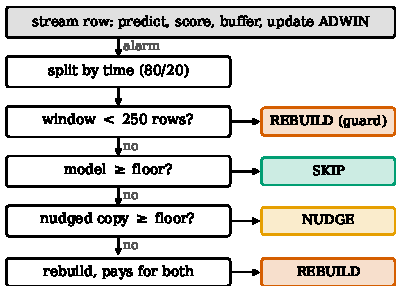
\includegraphics[width=\columnwidth]{figures/f1_decision_flow.pdf}
\caption{The selector's decision at one alarm.}
\label{fig:flow}
\end{figure}

Four baselines share identical mechanisms and the same temporal split, so a
difference between policies is attributable to the decision rule: NeverAdapt,
AlwaysRebuild, AlwaysNudge and FixedSchedule ($k=3$: nudge, nudge, rebuild).


\subsection{Cost accounting}

Training cost is $\textit{work units} = \textit{passes} \times \textit{rows}$. We
read the pass count from the fitted model, taking boosting rounds added, trees
added, \texttt{n\_iter\_} epochs, or one for a closed-form fit, rather than
assuming it; warm-started fits are counted as a delta against a snapshot taken
before the fit. Inference cost is counted per prediction: tree node visits for
XGBoost and Random Forest, from leaf depth per round and \texttt{decision\_path}
length per tree, and parameter reads for SGD and Gaussian NB. These units are
comparable within a family and not across families, and operation counts are not
joules.

\begin{algorithm}[t]
\caption{\textsc{MechanismSelector.adapt} at one alarm}
\label{alg:selector}
\small
\begin{algorithmic}[1]
\Require window $(X,y)$, reference accuracy $r$
\State $X_{tr},y_{tr},X_{ho},y_{ho} \gets$ \textsc{TemporalSplit}$(X,y,0.2)$
\State $\textit{floor} \gets r - 0.02$
\If{$|X_{ho}| < 50$ \textbf{or} $|X_{tr}| < 100$}
  \State \Return \textsc{Rebuild}$(X,y)$ \Comment{guard; charged in full}
\EndIf
\If{\textsc{Score}$(m,X_{ho},y_{ho}) \geq \textit{floor}$}
  \State \Return $m$ \Comment{SKIP, zero cost}
\EndIf
\State $c \gets$ \textsc{Nudge}$(\textsc{Copy}(m),X_{tr},y_{tr})$
\If{\textsc{Score}$(c,X_{ho},y_{ho}) \geq \textit{floor}$}
  \State \Return $c$ \Comment{NUDGE}
\EndIf
\State \Return \textsc{Rebuild}$(X,y)$ \Comment{charged for nudge $+$ rebuild}
\end{algorithmic}
\end{algorithm}

\subsection{The oracle}

At every alarm on the selector's real trajectory we snapshot the model, window,
reference and stream position, then execute all four branches (SKIP, NUDGE,
REBUILD, DEFER) from that snapshot. Each branch is scored over a horizon $H$,
taken as the rows to the next alarm and capped at 1{,}000, with $H=500$ and
$H=1{,}000$ as sensitivity checks. Each branch is charged
$\textit{Ops}(a)$ = training + evaluation + inference over the horizon, and the
cost of an action is
\begin{equation}
J(a) = \textit{Ops}(a) + \lambda\,\textit{Errors}(a),
\end{equation}
which we report over a grid of $\lambda$ rather than at one chosen value. $O_1$
is the best of SKIP, NUDGE and REBUILD, and $G_1 = \textit{cost(selector)} -
\textit{cost}(O_1)$. In a per-alarm frame DEFER coincides with SKIP, so $G_2$
cannot exceed $G_1$ in this design; we state that limitation rather than work
around it.

\subsection{WaitAndCheck and its pre-declared rules}

On an alarm, WaitAndCheck$(W)$ (Alg.~\ref{alg:wac}) takes no action and keeps
predicting for $W$ labelled rows. Further alarms are ignored and counted, the
detector is not reset, and the rows enter the buffer. The model is then scored on
exactly those $W$ rows with the floor's metric. If the score sits at or above the
floor, the alarm is cancelled at zero training cost; otherwise the enlarged
buffer goes to the unchanged selector. We set $W=200$ as primary and $W=500$ as
secondary.

Three rules were fixed before the runs: (1) training operations
$\leq 0.75\times$ the selector's on $\geq 4$ of 5 streams; (2) balanced accuracy
$\geq$ selector $-1$ point on $\geq 4$ of 5; and (3) a hard safety rule on
INSECTS gradual and incremental, where a failure makes the verdict NO regardless
of the others. Elec2 and Covertype motivated the experiment, so they are not
held-out evidence for it.

\begin{algorithm}[t]
\caption{\textsc{WaitAndCheck}$(W)$ around the selector}
\label{alg:wac}
\small
\begin{algorithmic}[1]
\State on alarm at row $i$: record it, take no action
\For{the next $W$ labelled rows}
  \State predict, reveal label, buffer the row, update the detector
  \State ignore and count any further alarm
\EndFor
\State $a \gets$ \textsc{Score}$(m,\text{those } W \text{ rows})$ \Comment{floor's metric}
\If{$a \geq r - 0.02$} \Comment{ConfirmMD3: $r-a \leq \Theta\sigma$}
  \State cancel the alarm \Comment{no training; buffer and reference as SKIP}
\Else
  \State \Return \textsc{MechanismSelector.adapt}(buffer incl.\ the $W$ rows, $r$)
\EndIf
\end{algorithmic}
\end{algorithm}

\subsection{Statistics}

XGBoost and Gaussian NB are deterministic at these settings, which we verified on
the grid, so their five seeds count as one observation. Blocks are
(stream $\times$ family $\times$ seed) with those two families at seed 0, which
gives $n=60$ overall and $n=12$ per stream. We use Friedman with Nemenyi, and
paired Wilcoxon signed-rank with Holm correction. We also report $n=20$, one
observation per cell, as a stricter check, and mark conclusions that do not
survive it.

We label results \textsc{[verdict]} when they are judged against rules fixed
before we saw the data, and \textsc{[diag]} when they are measurements that carry
no verdict. The thresholds in our decision rules are our own choices, not
standard values.

\section{Results}


\subsection{The selector does not win \textsc{[diag]}}

Table~\ref{tab:main} gives the per-stream picture for every policy, and
Fig.~\ref{fig:tradeoff} plots the same runs as cost against accuracy. Across the
500-run grid, Friedman finds no significant difference between the five policies
in mean prequential accuracy ($p=0.18$ at $n=60$; $p=0.45$ at $n=20$), while cost
separates them sharply ($p=2.9\times10^{-43}$). The selector is significantly
\emph{less} accurate than AlwaysRebuild (median $-1.3$ points of mean prequential
accuracy, balanced on multi-class streams; Holm $p=0.017$) and much cheaper
(cheaper in 51 of 57 non-tied blocks, rank-biserial $r=-0.96$). It is more
expensive than FixedSchedule at $n=60$ (Holm $p=0.0087$), though that result
survives neither the stricter $n=20$ check ($p=0.088$) nor the DDM replicate
($p=0.065$). Across 20 cells, never adapting at all was at least as accurate at
zero training cost in 10.

\begin{table*}[!t]
\caption{Main results per stream and policy: median whole-stream prequential
balanced accuracy (\%) and median training work units, taken over the twelve
(family $\times$ seed) blocks of each stream. Best accuracy per stream in bold.
WaitAndCheck and ConfirmMD3 are at $W=200$; ConfirmMD3 is a diagnostic
comparison with no verdict attached.}
\label{tab:main}
\centering\small
\setlength{\tabcolsep}{4pt}
\begin{tabular}{@{}lrrrrrrr@{}}
\toprule
& \multicolumn{1}{c}{NeverAdapt} & \multicolumn{1}{c}{AlwaysRebuild}
& \multicolumn{1}{c}{AlwaysNudge} & \multicolumn{1}{c}{FixedSchedule}
& \multicolumn{1}{c}{Selector} & \multicolumn{1}{c}{WaitAndCheck}
& \multicolumn{1}{c}{ConfirmMD3} \\
\midrule
\multicolumn{8}{l}{\emph{median balanced accuracy} (\%)} \\
Elec2 & 65.3 & 69.3 & 70.5 & 70.0 & 66.9 & 69.3 & \textbf{71.3} \\
Covertype & \textbf{72.7} & 56.1 & 69.6 & 50.9 & 51.9 & 49.3 & 61.0 \\
INSECTS abrupt & 52.7 & 54.8 & 49.5 & 39.7 & 42.8 & 55.8 & \textbf{56.6} \\
INSECTS gradual & 28.0 & 48.5 & 27.9 & 29.2 & 40.0 & \textbf{52.4} & 52.1 \\
INSECTS incremental & 21.2 & \textbf{57.3} & 23.6 & 40.5 & 56.0 & 54.1 & 54.1 \\
\midrule
\multicolumn{8}{l}{\emph{median training work units}} \\
Elec2 & 0 & 2{,}841{,}360 & 77{,}760 & 914{,}710 & 1{,}413{,}405 & 907{,}266 & 608{,}018 \\
Covertype & 0 & 6{,}916{,}800 & 164{,}920 & 1{,}950{,}798 & 5{,}727{,}920 & 3{,}091{,}552 & 2{,}740{,}467 \\
INSECTS abrupt & 0 & 986{,}400 & 18{,}916 & 240{,}720 & 224{,}400 & 662{,}900 & 624{,}000 \\
INSECTS gradual & 0 & 571{,}200 & 12{,}078 & 214{,}350 & 307{,}532 & 318{,}100 & 316{,}100 \\
INSECTS incremental & 0 & 315{,}500 & 9{,}600 & 58{,}100 & 223{,}900 & 137{,}050 & 107{,}100 \\
\bottomrule
\end{tabular}
\end{table*}

Pooling hides the structure. Within each stream the policies differ
significantly: adaptation gains 20.3 and 36.2 points of median accuracy over
NeverAdapt on INSECTS gradual and incremental, and loses 14.8 points on
Covertype. The pooled null is cancellation across streams, a Simpson's-paradox
effect, so every result below is reported per stream.


\begin{figure*}[!t]
\centering
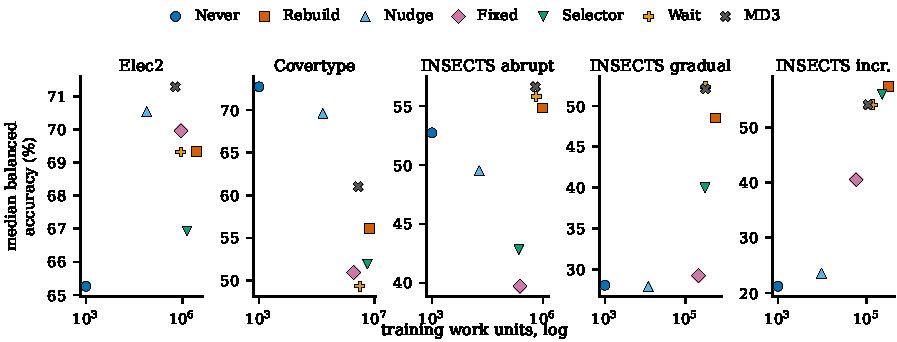
\includegraphics[width=\textwidth]{figures/f7_accuracy_cost.pdf}
\caption{Cost against accuracy per stream, one point per policy, over the twelve
(family $\times$ seed) blocks of each stream: median training work units against
median whole-stream prequential balanced accuracy. NeverAdapt trains nothing and
is drawn at the axis minimum. The ordering changes completely between streams.}
\label{fig:tradeoff}
\end{figure*}

\subsection{How cheap repair fails \textsc{[diag]}}

Of the selector's 2{,}830 adaptations, 841 were skips, 164 were kept nudges and
1{,}825 were rebuilds. Only 15.2\% of 1{,}079 nudge attempts cleared the floor.
Of the 915 failures, 69\% missed by more than 10 points, and in that group the
model was already a median 22.5 points below its floor when the alarm fired.

The failures differ in kind by family, which is visible once we look at
predictions rather than accuracy (Fig.~\ref{fig:nudge}). A Random Forest nudge
changed no prediction at all in 60\% of 1{,}876 nudges, and Gaussian NB in 77\%
of 364. SGD changed a median 9.4\% of predictions for a median accuracy gain of
0.0 points. Only XGBoost had a positive median gain, $+2.5$ points over 212
nudges. Refitting the nudge on the full window instead of the older 80\% leaves
this unchanged (median 0.00 points over 1{,}225 paired alarms; XGBoost $+2.28$).

\begin{figure*}[!t]
\centering
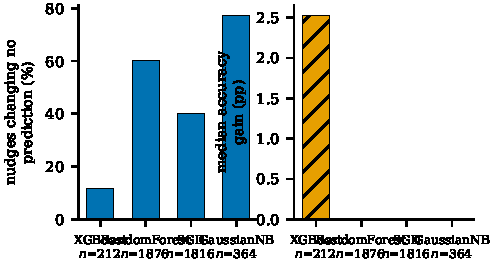
\includegraphics[width=\textwidth]{figures/f6_nudge_failure.pdf}
\caption{How a single nudge behaves, per family, under AlwaysNudge with ADWIN:
the share that changed no prediction at all (left) and the median accuracy gain
(right). $n$ is the number of nudges.}
\label{fig:nudge}
\end{figure*}

Half of the selector's rebuilds, 910 of 1{,}825, were forced by its own
minimum-window guard rather than by a failed nudge, which is 32\% of all its
adaptations. The runner clears the buffer after each adaptation, so an alarm that
follows closely arrives on a window too small to judge.

\subsection{What the alarms are \textsc{[diag]}}

On INSECTS-abrupt, whose change points are published~\cite{souza2020}, only
27.4\% of ADWIN alarms fall within 1{,}000 rows of one. The share rises with the
tolerance but stays a minority. Shuffling within blocks of 50 rows destroys local
label dependence and removes 40\% of ADWIN alarms and 69\% of DDM alarms on Elec2
and Covertype, where the error stream's lag-1 autocorrelation runs from $+0.58$
to $+0.90$ (Fig.~\ref{fig:alarms}).

\begin{figure}[t]
\centering
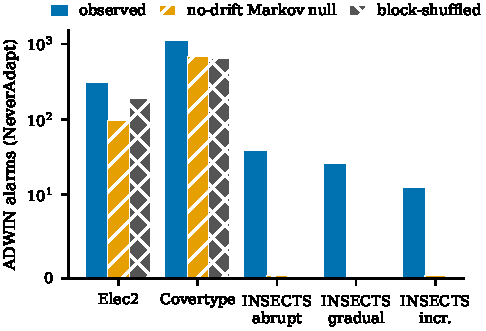
\includegraphics[width=\columnwidth]{figures/f2_alarm_validity.pdf}
\caption{ADWIN alarms with the model never changed: observed, under a no-drift
Markov null with the stream's own lag-1 dependence, and after shuffling within
blocks of 50 rows (Elec2 and Covertype only). Log scale.}
\label{fig:alarms}
\end{figure}

An i.i.d.\ null produced no ADWIN alarms at all, so we built a two-state Markov
null carrying each cell's own error rate and autocorrelation, with no drift
anywhere. It reproduces the observed falling-error share almost exactly, 0.421
against 0.416. The share of alarms that fire on a falling error rate is what such
a population produces.

We also tested each model against its own reference instead of comparing raw
estimates. By that test 38.1\% of 2{,}515 ADWIN alarms fired while the model was
significantly above the reference measured on the 200 rows after the previous
adaptation, or 36.5\% with an effective-sample-size correction, against the 5\%
the test yields by construction. Under DDM the same test gives 8.6\% and 3.5\%,
which is indistinguishable from the test's own rate, so this is an ADWIN result
only. The gap between the two detectors has a mechanism: DDM compares against the
minimum cumulative error since its own last reset, which sits below our reference
error in 79\% of its alarms by a median 14.7 points.

\subsection{The oracle: most of the gain is not acting \textsc{[diag]}}

On Elec2 and Covertype under ADWIN, over 2{,}595 alarms, $G_1$ is 16.8--25.5\%
and 24.8--37.1\% of the selector's cost respectively, across the whole $\lambda$
grid. Both are far above the 5\% we had set as the threshold below which no
decision model could help. Fig.~\ref{fig:oracle} shows where the advantage comes
from: SKIP accounts for 80.8\% of it on Covertype and 78.9\% on Elec2, NUDGE for
about 16\%, and REBUILD for 3--5\%.

\begin{figure}[t]
\centering
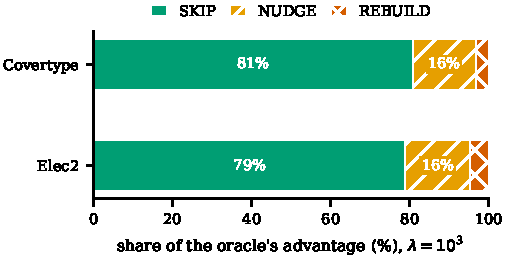
\includegraphics[width=\columnwidth]{figures/f3_oracle_branches.pdf}
\caption{Where the oracle's advantage over the selector comes from, per stream,
at $\lambda=10^3$, horizon ``next''. Segments below 8\% are not labelled: REBUILD
is 4.7\% on Elec2 and 3.3\% on Covertype.}
\label{fig:oracle}
\end{figure}

An ``always SKIP'' rule captures 95.3\% of $G_1$ at $\lambda=10^2$ and 78.1\% at
$\lambda=10^3$, but $-3.6\%$ at $\lambda=10^4$. Once errors are priced heavily
the choice of action starts to matter, and that is exactly where a fitted model
stops transferring: trained on one stream and tested on the other it captures
$-0.122$ and $+0.162$ of $G_1$ at $\lambda=10^4$. Within a stream across seeds it
holds up on Covertype (0.645) but not on Elec2 (0.085).

\subsection{What a repair costs after it is made \textsc{[diag]}}

Training work units and inference operations are different quantities, so we
report them on their own scales rather than as shares of a sum
(Fig.~\ref{fig:split}). Per-prediction inference cost ranges from 201 operations
for SGD to 4{,}009 for XGBoost under AlwaysNudge, and it is the one cost term a
repair changes permanently.

\begin{figure*}[!t]
\centering
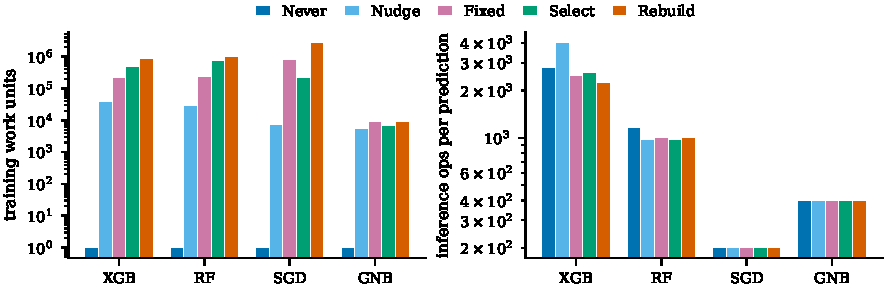
\includegraphics[width=\textwidth]{figures/f4_cost_split.pdf}
\caption{Cost on its two scales, by family and policy: training work units
(median per run, left) and inference operations per prediction (mean per run,
right). The two are different quantities and are never summed. Log axes, so
NeverAdapt, which trains nothing, is drawn at the axis minimum.}
\label{fig:split}
\end{figure*}

Adding boosting iterations is known to enlarge a model and hurt inference
throughput~\cite{lin2025}. We measured it per repair. Across the 32 kept XGBoost
nudges, 24 on Covertype, 5 on Elec2 and one on each of three INSECTS streams, the
nudge adds a median $+18.8$ to $+184.9$ node visits per prediction, measured
against a counterfactual rebuild fitted from the same snapshot. The Random Forest
add-$k$-retire-$k$ nudge adds $+4.8$, $+8.0$, $+1.3$, $-0.2$ and $-2.1$, so it
stays flat, as its design intends. It is a clean control only once growth is
separated from the window-size term. The sample is small, and we offer this as a
mechanism rather than as evidence about lifetime cost.

One related diagnostic is worth recording. Models rebuilt on 1{,}000-row windows
are cheaper to query than the initial model trained on 3{,}624--8{,}000 rows, but
a control model trained on 1{,}000 rows from the initial era is equally cheap.
The effect comes from the window size, not from rebuilding.

\subsection{WaitAndCheck \textsc{[verdict: no]}}
\label{sec:wac}


The verdict is \textbf{NO}. Every ratio and accuracy change in this section, in
Table~\ref{tab:md3} and in Fig.~\ref{fig:wac} is a median over the twelve
(family $\times$ seed) blocks of a stream, which is the statistic Rule 1 names.

\begin{figure}[t]
\centering
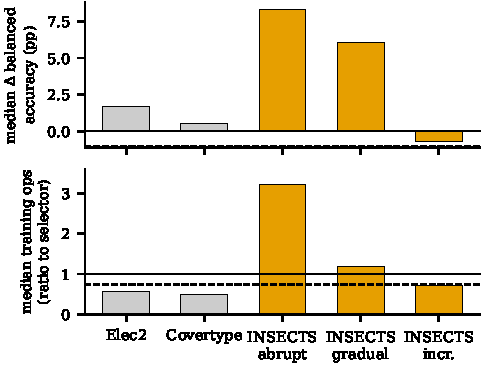
\includegraphics[width=\columnwidth]{figures/f5_waitandcheck.pdf}
\caption{WaitAndCheck ($W=200$) against the selector per stream: change in
balanced accuracy (top) and training operations as a ratio (bottom). Both are
medians over the twelve (family $\times$ seed) blocks of a stream, with a block
in which the selector performs no training counted as an undefined ratio ranked
above every finite one. Grey bars mark the two streams that motivated the
experiment and are not held-out evidence; dashed lines are our pre-declared
thresholds.}
\label{fig:wac}
\end{figure}

Under that statistic the five training ratios are 0.58 (Elec2), 0.49
(Covertype), 3.23 (INSECTS abrupt), 1.19 (INSECTS gradual) and 0.87 (INSECTS
incremental), so 2 of 5 streams reach $\leq 0.75\times$ and Rule 1 fails. One
detail deserves stating. In three INSECTS-incremental blocks the selector trains
nothing at all, so the ratio is undefined there. The computation used at decision
time ranked those blocks above every finite ratio, giving 0.87; dropping them
instead gives 0.71, which would make 3 of 5 streams pass. The pre-declared rule
named the statistic but not the treatment of an undefined block, so we report
both. Rule 1 fails either way, since neither reaches 4 of 5.

Rule 3 did not specify an accuracy statistic. INSECTS-incremental is $-1.07$
points on the mean and $-0.66$ on the median; the rule did not fix the statistic,
so Rule 3 fails under the mean and passes under the median. The verdict is NO
regardless, because Rule 1 fails under both. Rule 2 passes on 4 of 5 streams.

The diagnostic picture is more favourable, and we state it in full. Median
balanced accuracy rises on 4 of 5 streams, from $+0.55$ to $+8.34$ points, with a
pooled median of $+2.8$ (Holm $p=0.0004$) and per-stream significance on INSECTS
abrupt (Holm $p=0.0024$) and gradual (Holm $p=0.0098$). The gain does not come
mainly from cancelling alarms. Guard-forced rebuilds collapse from 752 to 40 on
Covertype and from 143 to 10 on Elec2 because the waited rows enlarge the repair
window, and INSECTS-abrupt is significantly worse on training (median
$+332{,}806$ work units, Holm $p=0.0024$) because each adaptation it still takes
runs over a bigger window. Cancelling also discards real drift: 23 of 79
cancelled alarms on INSECTS-abrupt fall within 1{,}000 rows of a published change
point. On Covertype WaitAndCheck loses to NeverAdapt by 8.6 points of balanced
accuracy.

\textbf{An MD3-style cancel rule \textsc{[diag]}.} To separate the waiting from
the cancel rule, we re-ran the same grid with one change: cancel unless the drop
in accuracy exceeds $\Theta$ standard errors of the reference estimate, that is
$\textit{reference}-\textit{acc}_W \leq \Theta\sigma$ with $\Theta=2$ and
$\sigma=\sqrt{p(1-p)/W}$ for $p$ the reference accuracy. This approximates
MD3~\cite{sethi2017}, which uses $Acc_{Ref}-Acc_{Labeled} > \Theta\sigma_{Acc}$
with $\sigma$ estimated from training data. Our $\sigma$ comes from the reference
estimate over the $W$ rows, and on multi-class streams the metric is balanced
accuracy, for which the binomial standard error is only approximate. We attach no
verdict to it, because the pre-declared rules were written for WaitAndCheck.

The looser rule cancels more and trains less than WaitAndCheck on every stream
(Table~\ref{tab:md3}). Paired against WaitAndCheck, the training reduction is
significant after Holm correction at $W=500$ on Covertype ($p=0.049$) and Elec2
($p=0.023$), but not at $W=200$. Neither failure behind the verdict is rescued:
INSECTS-abrupt still trains $2.76\times$ the selector, and INSECTS-incremental
falls further below it in accuracy, at $-2.44$ points. Covertype is the
exception, cheaper and 8.7 points more accurate than WaitAndCheck, on a stream
that is not held-out evidence.

\begin{table}[t]
\caption{ConfirmMD3 ($\Theta=2$) beside WaitAndCheck, $W=200$: training as a
ratio to the selector and the change in balanced accuracy, both as medians over
blocks (\S\ref{sec:wac}).}
\label{tab:md3}
\centering\small
\begin{tabular}{lcccc}
\toprule
& \multicolumn{2}{c}{WaitAndCheck} & \multicolumn{2}{c}{ConfirmMD3} \\
\cmidrule(lr){2-3}\cmidrule(lr){4-5}
Stream & train & $\Delta$acc & train & $\Delta$acc \\
\midrule
Elec2 & 0.58 & $+1.72$ & 0.51 & $+2.76$ \\
Covertype & 0.49 & $+0.55$ & 0.43 & $+9.24$ \\
INSECTS abrupt & 3.23 & $+8.34$ & 2.76 & $+5.59$ \\
INSECTS gradual & 1.19 & $+6.04$ & 0.92 & $+5.19$ \\
INSECTS incremental & 0.87 & $-0.66$ & 0.60 & $-2.44$ \\
\bottomrule
\end{tabular}
\end{table}

\section{Discussion}

Four things follow for a practitioner. The first is to adapt less on streams like
Elec2 and Covertype, where the largest single lever in the oracle is skipping
alarms and never adapting was at least as accurate as the adaptive policies, at
zero training cost, in half the cells. That advice does not generalise: on
INSECTS gradual and incremental, adaptation gains 20.3 and 36.2 points of median
balanced accuracy over NeverAdapt, and skipping would be the wrong default.

The second is to check what the detector is reacting to. A large share of the
alarms we see is produced by temporal dependence rather than by concept change,
which is a property of these benchmarks as much as of the detectors.

The third is to count inference alongside training. A repair that grows the model
raises the cost of every later prediction, and a training-only account cannot see
that happening.

The fourth concerns the repair window. Most of WaitAndCheck's accuracy gain came
from adapting on larger windows rather than from cancelling alarms, which makes
the window the repair sees worth studying on its own.

\section{Limitations}

Our evidence covers five streams, one configuration of each detector (ADWIN
$\delta=0.002$ two-sided on the raw error stream; DDM at library defaults), and
four model families. We count operations, not joules, so our cost numbers cannot
be converted to energy.

Training work units and inference operations are different quantities and are not
converted to a common scale. The oracle's $\textit{Ops}$ term sums them; our
$\lambda$ grid varies the weight of operations against errors but not the weight
of training against inference, so the SKIP decomposition is untested under other
weightings.

Several results rest on small samples. The selector kept only 164 nudges, of
which 32 were XGBoost, so the growth analysis is thin. The oracle decides per
alarm with foresight, which makes it an upper bound, and DEFER coincides with
SKIP in that frame, so the guard question it was meant to answer remains
untested. The oracle and its learnability analysis cover two streams only.
XGBoost and Gaussian NB are deterministic at these settings, so the effective
sample is 12 blocks per stream and 60 overall rather than 100.

Three further caveats apply to specific numbers. Elec2 and Covertype motivated
WaitAndCheck and are not held-out evidence for it. Inference totals between two
measured endpoints are interpolated from the logged size trajectory. The
MD3-style comparison uses our own approximation of $\sigma$ and a single
$\Theta$, runs on the same five streams, and carries no verdict. Nothing here
should be read as a statement about detectors or repairs outside these
configurations.

\section{Conclusion}

We measured what happens after a drift alarm, using operation counts for training
and for inference, a frozen grid, and an oracle. A cost-ordered
try-cheap-repair-first policy is not the best choice. Most of the oracle's
advantage lies in not acting. The alarms are largely explained by temporal
dependence on these benchmarks. A repair that grows the model raises the cost of
every later prediction, and a confirm-before-acting rule improved balanced accuracy
while failing the cost and safety rules we had fixed in advance.

Three things would extend this work. An MD3-style confirmation rule deserves
pre-declared rules of its own, with $\Theta$ and $\sigma$ treated as design
choices rather than fixed as they are here. Repair-window size deserves a
declared experiment, since it appears to drive the accuracy effect we had
attributed to waiting. More streams would help, including synthetic generators
with known change points and stationary controls, where a false alarm is false by
construction.

\section*{Artifact}

Code, the frozen grids, every analysis file, and a claims ledger mapping each
number in this paper to its source are available in the project repository.

\bibliographystyle{IEEEtran}
\bibliography{refs}

\end{document}
